\documentclass[12pt]{article}

\usepackage[margin=1in]{geometry}
\usepackage{mathptmx}
\usepackage{graphicx}
\usepackage{amsmath}
\usepackage{booktabs}
\usepackage{caption}
\usepackage{float}
\usepackage{xcolor}
\usepackage{listings}
\usepackage[hidelinks]{hyperref}
\usepackage{titlesec}

\titleformat{\section}[block]
{\normalfont\bfseries}
{}
{0pt}
{\underline}

\renewcommand{\figurename}{FIGURE}
\renewcommand{\tablename}{TABLE}
\renewcommand{\contentsname}{Table of Contents:}
\renewcommand{\listfigurename}{List of Figures:}
\renewcommand{\baselinestretch}{1.15}

\captionsetup[figure]{labelfont=bf,labelsep=period}
\captionsetup[table]{labelfont=bf,labelsep=colon}

\lstdefinelanguage{VHDL}{
  morekeywords={
    library,use,entity,architecture,is,begin,end,port,generic,signal,constant,
    process,if,then,elsif,else,case,when,others,loop,for,while,wait,until,
    in,out,inout,map,downto,to,of,type,record,function,return,report,severity,
    component,array,variable,package,body
  },
  sensitive=false,
  morecomment=[l]--,
  morestring=[b]"
}

\lstdefinestyle{vhdlstyle}{
  language=VHDL,
  basicstyle=\ttfamily\scriptsize,
  keywordstyle=\color{blue!70!black}\bfseries,
  commentstyle=\color{green!40!black},
  stringstyle=\color{red!50!black},
  numbers=left,
  numberstyle=\tiny\color{gray},
  stepnumber=1,
  numbersep=8pt,
  breaklines=true,
  breakatwhitespace=false,
  showstringspaces=false,
  frame=single,
  tabsize=2
}

\graphicspath{{Images/}}

\begin{document}

\thispagestyle{empty}
\begin{center}
  {\Huge \bfseries ELEG 4593/5593: Programming for Power Electronics\par}

  \vspace{2cm}

  {\Large Final Project: Serial, SPRAM, PWM, ADC, and PID Buck Converter Control\par}

  \vspace{3cm}
\end{center}

\vfill
\begin{flushright}
  Kevin Lyon\\[0.5cm]
  ELEG 4593\\
  Final Project\\
  03 May 2026
\end{flushright}
\newpage

\setcounter{page}{2}

\section*{Abstract:}
\addcontentsline{toc}{section}{Abstract:}

This final project expands the earlier UART, SPRAM, PWM, and ADC design into a closed-loop buck converter controller. The completed system uses the LabVIEW serial interface to write and read memory-mapped registers, samples the Small PE-Eval Board feedback signals with the AD7928 ADC, and drives the buck converter gate signal \texttt{DSP\_G1} from a dedicated PID-controlled PWM output. The PID controller is implemented as a reusable fixed-point module and is connected to the rest of the project through a SPRAM wrapper. The wrapper reads the PWM enable, setpoint, feedback, PWM divider, and PID coefficients from SPRAM, executes one PID step at the ADC sweep rate, and converts the signed PID output into a 12-bit PWM duty command. Hardware testing showed working ADC readback and closed-loop control of the buck output.

\newpage

\begingroup
\let\clearpage\relax
\tableofcontents
\vspace{1em}
\listoffigures
\vspace{1em}
\listoftables
\endgroup

\newpage

\section*{Assignment Summary}
\addcontentsline{toc}{section}{Assignment Summary}

The final assignment required the Homework~9 serial/register/PWM/ADC interface to be expanded so that it controlled the Small PE-Eval Board's buck converter. The required top-level ports were the UART input and output, the AD7928 SPI pins, four LED/PWM outputs, and the buck gate drive output \texttt{DSP\_G1}. The extra-credit closed-loop requirement was to incorporate a simple PI controller, include the source code in the appendix, and show hardware ADC values for the buck output.

The implemented design keeps the same general architecture used in the previous assignments. UART packets from LabVIEW are decoded by the serial controller and converted into SPRAM read/write transactions. The PWM client, ADC client, PID wrapper, and UART controller share the same SPRAM through a fixed-priority \texttt{Bus\_Master}. The ADC client periodically stores the latest AD7928 readings beginning at address \texttt{0x0200}, and the PID wrapper uses the \texttt{V\_Buck} \textit(0x0201) feedback register as its measured process value.

\section*{System Architecture}
\addcontentsline{toc}{section}{System Architecture}

The top-level file, \texttt{uart\_spram\_top.vhd}, granted a name no longer fitting of the top module but the result of how things evolved, instantiates the internal oscillator, PLL, reset delay, UART controller, four-channel LED PWM client, ADC client, PID wrapper, \texttt{Bus\_Master}, and generated SPRAM block. The \texttt{Bus\_Master} uses fixed priority arbitration:

\begin{itemize}
  \item Client 0: \texttt{pwm\_spram\_client}
  \item Client 1: \texttt{pid\_spram\_pwm\_wrapper}
  \item Client 2: \texttt{adc\_spram\_client}
  \item Client 3: \texttt{uart\_rs232\_fifo\_wrap\_controller}
\end{itemize}

\noindent The LED PWM client continues to read the LED control block beginning at \texttt{0x0100}. In this final version, \texttt{LED1\_Intensity} is also used as the PID setpoint register. The ADC client writes each 12-bit ADC result into a 16-bit SPRAM word beginning at \texttt{0x0200}. The PID wrapper then reads the PWM enable bit, PWM divider, coefficients, feedback, and setpoint from SPRAM before each PID calculation.

\begin{table}[H]
  \centering
  \caption{Final project memory map used by the PID and ADC system.}
  \label{tab:memory-map}
  \begin{tabular}{lll}
    \toprule
    Address & Register & Use \\
    \midrule
    \texttt{0x0100} & PWM enable & Enables LED PWM outputs and manual integrator reset \\
    \texttt{0x0101} & PWM frequency control & Controlled by LabVIEW \texttt{LED\_BlinkPRD} \\
    \texttt{0x0103} & PID setpoint & Shared with \texttt{LED1\_Intensity} \\
    \texttt{0x0200}--\texttt{0x0207} & ADC samples & Latest AD7928 channel results \\
    \texttt{0x0201} & PID feedback & \texttt{V\_Buck} feedback used by the PID loop \\
    \texttt{0x0300} & \texttt{Kp} & Proportional coefficient \\
    \texttt{0x0301} & \texttt{Ki} & Integral coefficient \\
    \texttt{0x0302} & \texttt{Kd} & Derivative coefficient \\
    \texttt{0x0310}--\texttt{0x0314} & PID debug & Setpoint, feedback, error, output, duty \\
    \texttt{0x0315}+ & Integrator debug & Full value, 16-bit words, MSB first \\
    \bottomrule
  \end{tabular}
\end{table}

\section*{PID Implementation}
\addcontentsline{toc}{section}{PID Implementation}

The PID algorithm is implemented in \texttt{My\_PID.vhd}. The core runs one calculation each time \texttt{execute\_i} receives a rising edge. It does not continuously recompute between execute pulses. The error input is signed, while \texttt{Kp}, \texttt{Ki}, and \texttt{Kd} are unsigned fixed-point values. In this build, the coefficients use 10 fractional bits, so the real coefficient is

\begin{equation}
  \mathrm{gain} = \frac{\mathrm{register\ value}}{2^{10}}.
\end{equation}

\noindent The PID terms are calculated as

\begin{equation}
  P = e \cdot K_p,
  \qquad
  I = (accumulator \gg 8) \cdot K_i,
  \qquad
  D = (e - e_{previous}) \cdot K_d.
\end{equation}

\noindent The integrator shift of 8 is set in the top-level file when the PID wrapper is instantiated. That shift does not change the stored accumulator, but rather only reduces the accumulator's contribution to the PID output as we usually want a very small integral term and I didn't much fancy having separate gain dividers for $K_p$, $K_i$, and $K_d$. The following default coefficients are written into SPRAM by the PID wrapper once after reset:

\begin{table}[H]
  \centering
  \caption{Default PID coefficients written at startup.}
  \label{tab:pid-gains}
  \begin{tabular}{llll}
    \toprule
    Coefficient & Address & Default Hex & Default Real Gain \\
    \midrule
    \texttt{Kp} & \texttt{0x0300} & \texttt{0x0050} & 0.078125 \\
    \texttt{Ki} & \texttt{0x0301} & \texttt{0x0005} & 0.0048828125 \\
    \texttt{Kd} & \texttt{0x0302} & \texttt{0x0000} & 0.0 \\
    \bottomrule
  \end{tabular}
\end{table}

\noindent Since \texttt{Kd} is zero by default, the implemented controller is operating as a PI controller unless a nonzero derivative coefficient is written through the serial interface.  I put \textbf{ZERO} time into tuning this PID controller.  As it is running much faster than the serial communications I would need to feed the output into an oscilloscope to tune it.  It is sitting on my desk.  The Scope is across the hall.  It was...so far.  I was grateful you didn't require us to spend that 10 minutes.  However I am quite confident that my available parameter range would allow for a solidly tuned PID response.  

\section*{PID Wrapper Operation}
\addcontentsline{toc}{section}{PID Wrapper Operation}

The file \texttt{pid\_spram\_pwm\_wrapper.vhd} connects \texttt{My\_PID} to the shared SPRAM bus and to a dedicated PWM generator. The wrapper first writes the default coefficients into \texttt{0x0300}--\texttt{0x0302}. After startup, it waits for its fixed update timer, then performs seven SPRAM reads: PWM enable, PWM frequency control, \texttt{Kp}, \texttt{Ki}, \texttt{Kd}, feedback, and setpoint. The update timer is hardwired from the top level to match the ADC sweep period. The setpoint comes from address \texttt{0x0103}, which corresponds to the LabVIEW \texttt{LED1\_Intensity} control. The feedback comes from address \texttt{0x0201}, which is the memory-mapped \texttt{V\_Buck} ADC channel used for closed-loop control.

The setpoint is a 16-bit LabVIEW value, while the ADC feedback is a 12-bit value stored in a 16-bit word. To simply map them into the same width, the wrapper uses the upper 12 bits of the setpoint:

\begin{equation}
  setpoint_{ADC} = setpoint(15 \; downto \; 4).
\end{equation}

\noindent The error is then formed as

\begin{equation}
  error = setpoint_{ADC} - feedback.
\end{equation}

\noindent After pulsing \texttt{execute\_i}, the wrapper waits for the pipelined PID output to update. Negative PID output is clipped to zero, and positive output is saturated to the 12-bit PWM range. That 12-bit duty command drives a separate \texttt{pwm\_generic} instance whose output is connected directly to \texttt{DSP\_G1}. The LED PWM outputs are active-low at the top-level, but \texttt{DSP\_G1} is not inverted. If the PWM enable bit at \texttt{0x0100} is zero, the wrapper skips the PID execute pulse, forces the duty to zero, and clears the PID accumulator so re-enabling PWM from LabVIEW behaves like a manual integral reset.

The LabVIEW \texttt{LED\_BlinkPRD} slider is reused as a bounded PWM frequency control for both the LED PWM block and the buck converter PWM. Like the other LabVIEW controls, it uses the full 16-bit range from 0 to 65535. It does not create a blink envelope. A value of 0 gives the fastest 12-bit PWM rate, approximately 6.09~kHz with the 24.93~MHz system clock. A value of 65535 maps to an effective divider of 6, or approximately 1.01~kHz. The mapping is intentionally bounded so the slider cannot accidentally force the buck converter into an unreasonable low-frequency switching mode. The PWM frequency is

\begin{equation}
  f_{PWM} = \frac{24.93~\mathrm{MHz}}{\mathrm{effective\ divider} \cdot 2^{12}}.
\end{equation}

\noindent The PID executes once per ADC sweep period so it does not integrate the same stale feedback value repeatedly. The first LED output is also driven from the PID PWM signal, so \texttt{LED1} mirrors the buck converter duty cycle and gives a visible indication that the PID output is changing.

\section*{Serial Commands For PID Coefficients}
\addcontentsline{toc}{section}{Serial Commands For PID Coefficients}

The UART packet format is

\begin{center}
\texttt{7E | LEN | OP\_ID | COUNT | ADDR\_H | ADDR\_L | DATA... | CHKSUM}
\end{center}

\noindent where \texttt{0x0A} is the write command, \texttt{0x0F} is the read command, and the checksum is \texttt{0xFF} minus the 8-bit sum of the payload bytes. Example coefficient packets are shown in Table~\ref{tab:packets}.

\begin{table}[H]
  \centering
  \caption{Example UART packets for reading or changing PID coefficients.}
  \label{tab:packets}
  \begin{tabular}{ll}
    \toprule
    Purpose & Packet Bytes \\
    \midrule
    Read \texttt{Kp}, \texttt{Ki}, \texttt{Kd} & \texttt{7E 04 0F 03 03 00 EA} \\
    Write \texttt{Kp = 0x0050} & \texttt{7E 06 0A 01 03 00 00 50 A1} \\
    Write \texttt{Ki = 0x0005} & \texttt{7E 06 0A 01 03 01 00 05 EB} \\
    Write \texttt{Kd = 0x0000} & \texttt{7E 06 0A 01 03 02 00 00 EF} \\
    Write all defaults at once & \texttt{7E 0A 0A 03 03 00 00 50 00 05 00 00 9A} \\
    Write PWM frequency control full-scale & \texttt{7E 06 0A 01 01 01 FF FF F4} \\
    \bottomrule
  \end{tabular}
\end{table}

\section*{Hardware Results}
\addcontentsline{toc}{section}{Hardware Results}

Figure~\ref{fig:pid-running-low} shows the LabVIEW interface with the PID system running and the buck output reading approximately 1.66~V. The \texttt{V\_Pot} readout is present and scaled correctly, confirming that the ADC path is working through the serial/SPRAM interface. The \texttt{V\_Buck} readout is the feedback value used by the PID loop.

\begin{figure}[H]
  \centering
  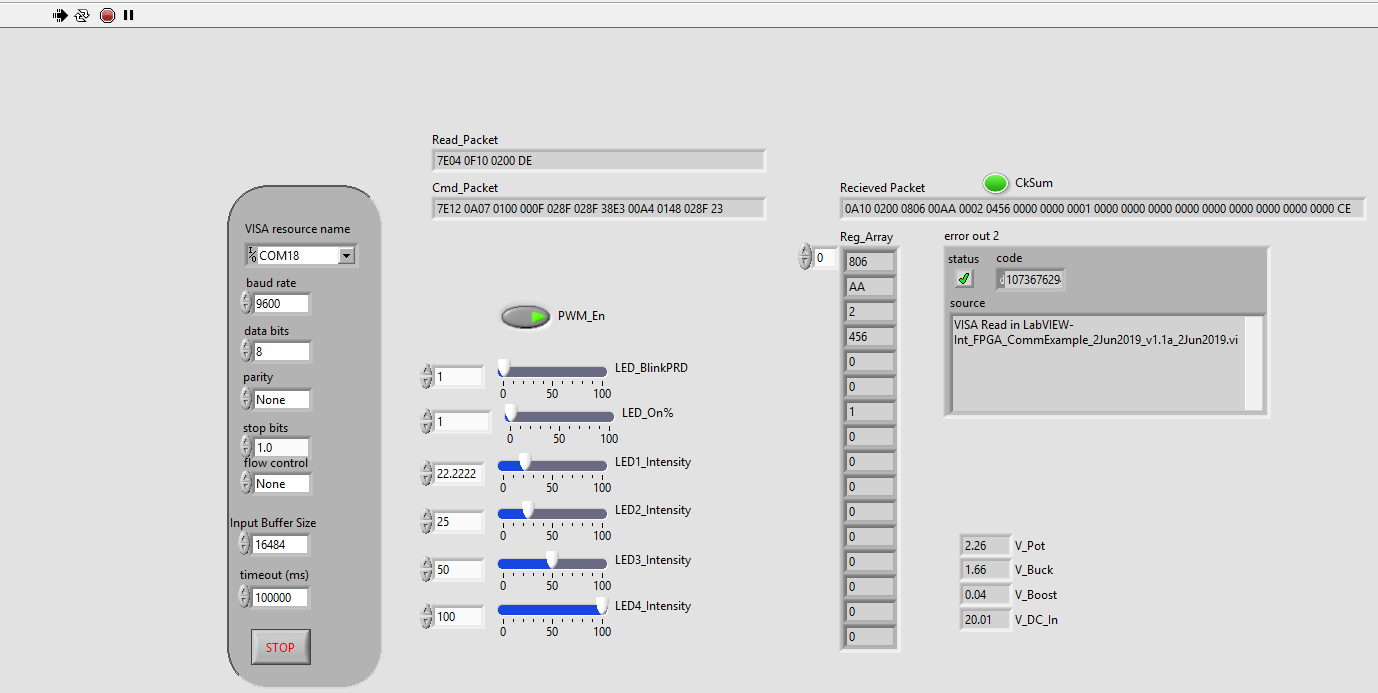
\includegraphics[width=\textwidth]{RunningPID1_5V.png}
  \caption{LabVIEW hardware readback with the PID-controlled buck converter running.}
  \label{fig:pid-running-low}
\end{figure}

Figure~\ref{fig:pid-running-high} shows a second operating point with a higher \texttt{LED1\_Intensity} setpoint and a measured \texttt{V\_Buck} value of approximately 3.32~V. This demonstrates that the LabVIEW setpoint control is affecting the converter output and that the ADC values are being returned to the host interface.

\begin{figure}[H]
  \centering
  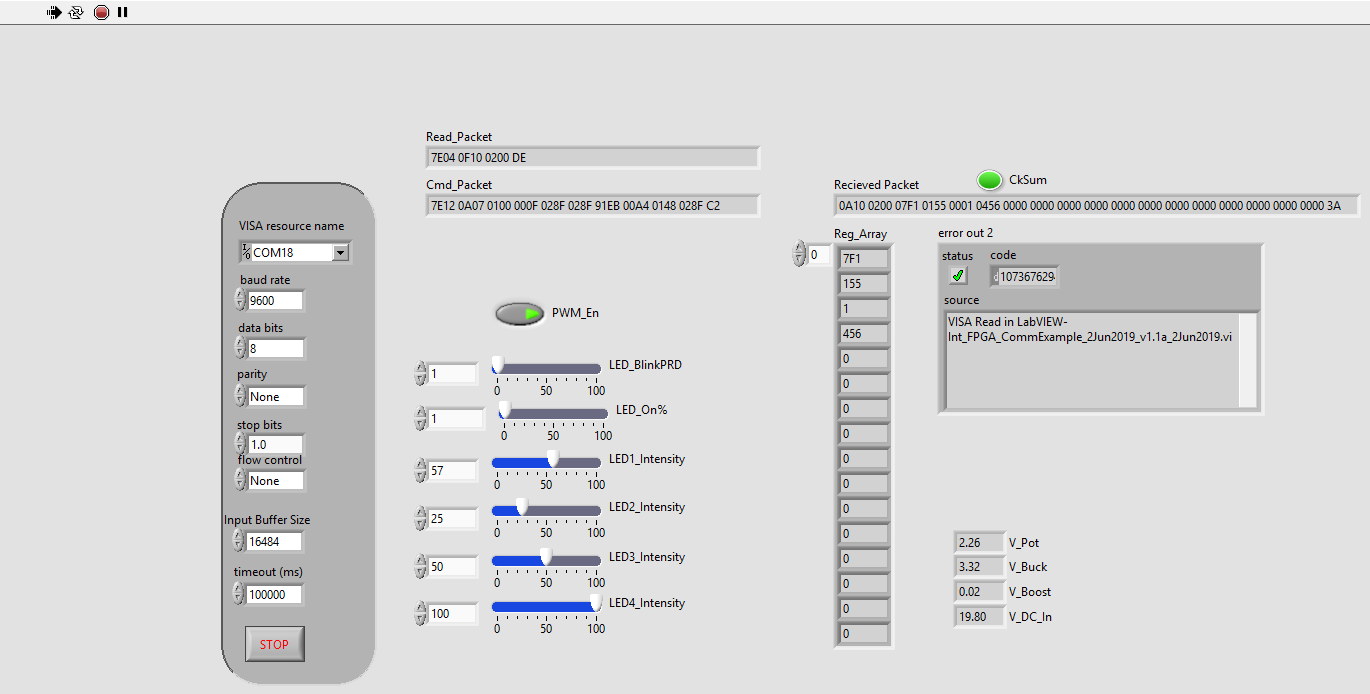
\includegraphics[width=\textwidth]{RunningPID.png}
  \caption{LabVIEW hardware readback at a higher PID setpoint.}
  \label{fig:pid-running-high}
\end{figure}

\section*{Integrator Behavior}
\addcontentsline{toc}{section}{Integrator Behavior}

During hardware testing before the final timing change, the loop showed integrator spool-up and could slowly lose lock over time. The final code uses a 12-bit PWM period for the controlled outputs, so the fastest PWM timing reference is about

\begin{equation}
  \frac{24.93~\mathrm{MHz}}{2^{12}} \approx 6.09~\mathrm{kHz}.
\end{equation}

\noindent The earlier problem occurred when the PID could execute many times per ADC refresh and integrate the same stale feedback error repeatedly. The PID core does saturate its internal accumulator and output width, but the wrapper does not implement true anti-windup based on the final PWM duty saturation. Therefore, when the duty command rails high or low, the integrator may continue accumulating and then require time to unwind. This is especially noticeable if the setpoint slider is pulled all the way to full scale. In that case, the controller can demand more output than the buck converter can produce, so the integral term spools up aggressively while the PWM duty is already saturated.

\noindent A second spool condition showed up in hardware when the commanded buck voltage was set to zero. In that case the feedback remains positive while the setpoint is zero, so the error tends to stay negative. The integrator can then spool in the negative direction and make the later response feel sluggish when the setpoint is increased again, because the controller must first unwind that stored negative integral before the output rises. The final wrapper revision therefore uses the PWM enable bit at \texttt{0x0100} as a practical manual reset control: disabling PWM forces the duty cycle to zero and clears/holds the integrator, while re-enabling PWM lets the controller restart from a clean state. This is not a substitute for full anti-windup logic, but it does give the LabVIEW interface a simple and useful recovery tool during testing and was fast to implement.

\section*{Conclusion}
\addcontentsline{toc}{section}{Conclusion}

The final project successfully combines the UART register interface, shared SPRAM bus, LED PWM client, AD7928 ADC client, and a fixed-point PID controller to drive the Small PE-Eval Board buck converter. The design meets the required serial, ADC, PWM, and \texttt{DSP\_G1} control functions, and the included LabVIEW screenshots show live ADC readback from the running hardware. The PID implementation is memory-mapped and tunable through the same UART packet interface used throughout the course. The final revision ties the PID calculation rate to the ADC sweep rate while leaving the former \texttt{LED\_BlinkPRD} register available as a bounded PWM frequency control for both the LEDs and the buck converter. The first LED is driven from the same PID PWM duty as \texttt{DSP\_G1}. Disabling the PWM enable bit now also clears and holds the integrator, which gives the LabVIEW front end a simple manual reset option when the loop has spooled in either direction. Future work should still add true anti-spooling/anti-windup logic so the integral term stops accumulating automatically when the commanded duty cycle has already reached its usable limit.

\appendix

\section*{Appendix A: Source Code Listings}
\addcontentsline{toc}{section}{Appendix A: Source Code Listings}

The following listings include the handwritten source files relevant to the final project. The generated SPRAM and PLL files are omitted because they are tool-generated. No testbench is included for this final report.

\subsection*{A.1 uart\_spram\_top.vhd}
\lstinputlisting[style=vhdlstyle]{uart_spram_top.vhd}

\subsection*{A.2 pid\_spram\_pwm\_wrapper.vhd}
\lstinputlisting[style=vhdlstyle]{pid_spram_pwm_wrapper.vhd}

\subsection*{A.3 My\_PID.vhd}
\lstinputlisting[style=vhdlstyle]{../PID_Module/My_PID.vhd}

\subsection*{A.4 PWM\_Module.vhd}
\lstinputlisting[style=vhdlstyle]{../PWM_Module/PWM_Module.vhd}

\subsection*{A.5 bus\_pkg.vhd}
\lstinputlisting[style=vhdlstyle]{bus_pkg.vhd}

\subsection*{A.6 Bus\_Master.vhd}
\lstinputlisting[style=vhdlstyle]{Bus_Master.vhd}

\subsection*{A.7 pwm\_spram\_client.vhd}
\lstinputlisting[style=vhdlstyle]{pwm_spram_client.vhd}

\subsection*{A.8 adc\_spram\_client.vhd}
\lstinputlisting[style=vhdlstyle]{adc_spram_client.vhd}

\subsection*{A.9 uart\_rs232\_fifo\_wrap\_controller.vhd}
\lstinputlisting[style=vhdlstyle]{uart_rs232_fifo_wrap_controller.vhd}

\subsection*{A.10 UART\_rs232\_fifo\_wrap.vhd}
\lstinputlisting[style=vhdlstyle]{UART_rs232_fifo_wrap.vhd}

\subsection*{A.11 UART\_rs232.vhd}
\lstinputlisting[style=vhdlstyle]{UART_rs232.vhd}

\subsection*{A.12 My\_Own\_FN\_FIFO.vhd}
\lstinputlisting[style=vhdlstyle]{My_Own_FN_FIFO.vhd}

\subsection*{A.13 AD7928\_Core.vhd}
\lstinputlisting[style=vhdlstyle]{../AD7928_core/AD7928_Core.vhd}

\end{document}
